%%%%%%%%%%%%%%%%%%%%%%%%%%%%%%%%%%%%%%%%%%%%%%%%%%%%%%%%%%
%% HEIG-VD / institut REDS
%%
%% Modèle Latex pour laboratoire
%% 
%% Fichiers à changer : 
%%            - constantes.tex
%%            - Tous les fichiers du corps du rapport 
%%
%% Auteur : MIM
%% Date   : 27.09.2017
%%%%%%%%%%%%%%%%%%%%%%%%%%%%%%%%%%%%%%%%%%%%%%%%%%%%%%%%%%

% Paramétrage du papier utilisé
\documentclass[a4paper,12pt,oneside]{article}

% Ne pas toucher, nécessaire à la mise en forme
\usepackage[utf8]{inputenc} 
\usepackage[T1]{fontenc} % Nouvelle norme pour codage des caractères
\usepackage{lmodern} % Nouvelle forme de la fonte ComputerModern
\usepackage[provide=*,french]{babel} % Règles typographiques françaises, césures
\usepackage{graphicx} % Insertion images
\usepackage{epstopdf} % Convertir les images eps vers pdf
\epstopdfsetup{outdir=./Images/converted_to_pdf/} % Dossier de sortie des images converties
\pagenumbering{arabic}
\usepackage[top=3cm, bottom=3cm, left=3cm, right=3cm, showframe=false]{geometry}
\usepackage{amsmath}
\usepackage{hyperref}
\usepackage{pdfpages}
\usepackage{pdflscape}
\usepackage{color}
\usepackage{float}
\usepackage{tabularx}
\usepackage{array}
% Package karnaugh-map inutilisé dans ce rapport.
\usepackage{caption}
\usepackage[table]{xcolor}
\usepackage{multicol} 
\usepackage{makecell}
\usepackage{subcaption}


\usepackage{booktabs}
\usepackage{multirow}
\usepackage{colortbl}
\usepackage{amsthm}
\usepackage{enumitem}
\usepackage{tikz}





% fichier avec les constantes (à adapter pour les étudiants)
%%%%%%%  Constantes (à changer) %%%%%%%%

\newcommand{\nomAuteur}{Gabriel Conde \& Elisa Dahman}

\newcommand{\titre}{Driver MOSFET et Snubber}

\newcommand{\nbrlabo}{2} % numéro de laboratoire

\newcommand{\prof}{Siemaszko Daniel}

\newcommand{\assistant}{Sefaranga Eliott} % 

\newcommand{\classe}{ElPui-2}

\newcommand{\departement}{Technologies industrielles (TIN)}

\newcommand{\cours}{Electronique de Puissance 2 (ElPui2)}


% Entête et pieds de page (A ADAPTER)
\pagestyle{empty}
\usepackage{fancyhdr}
\setlength{\headheight}{27.06pt}
\pagestyle{fancy}
% Entête :
\renewcommand{\headrulewidth}{1pt}
\fancyhead[L]{Labo\nbrlabo: \titre} 
\fancyhead[R]{Rapport de laboratoire} 
% Pied de page
\fancyfoot{} % clear all footer fields
\renewcommand{\footrulewidth}{1pt}
\fancyfoot[R]{Page \thepage} 
\fancyfoot[L]{HEIG-VD | \nomAuteur }

\setlength{\parindent}{0pt}

% Ajouts de contenu : figures vectorielles et références.
\usetikzlibrary{arrows.meta,positioning,calc}
\emergencystretch=2em
\renewcommand{\arraystretch}{1.15}
\hypersetup{hidelinks}
% debut du corps du rapport 
\begin{document}	
	% première page
	%%%%%%%%%%%%%%%%%%%%%%%%%%%%%%%%%%%%%%%%%%%%%%%%%%%%%%%%
% Ce document ne doit pas être modifié
% Il faut modifier les informations depuis le fichier
% constantes.tex
%%%%%%%%%%%%%%%%%%%%%%%%%%%%%%%%%%%%%%%%%%%%%%%%%%%%%%%%

\begin{center}

\includegraphics[height=2cm]{./images/logo_heig.pdf}
\hfill 
\includegraphics[height=2cm]{./images/logo_hesso.pdf}
\end{center}

\vfill

\begin{center}
	\Large Laboratoire \nbrlabo: \\
	\huge \titre \\
\end{center}


\begin{center}
	\begin{tabular}{l l}
		Département:          & \departement\\
		Unité d'enseignement: & \cours\\
	\end{tabular}
\end{center}


\vfill

\begin{center}
    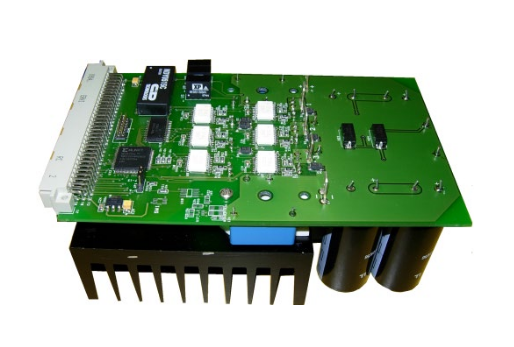
\includegraphics{images/circuit.png}
\end{center}

\vfill

\begin{tabular}{l l}
	\Large	Auteurs:   			  & \Large \nomAuteur\\
	Professeur:           & \prof\\
	Assistant:			  & \assistant\\
	Classe:               & \classe\\
	Date:                 & \today\\
\end{tabular}

\vfill

\begin{center}

\includegraphics[height=2 cm]{images/IE.png}
\end{center}
\newpage

\tableofcontents
\newpage

	% enlève le numero sur la premiere page
	% En-têtes du modèle conservés pour le corps du rapport.
	% Pagination continue après la couverture et la table des matières.
	\newpage
	

    \section*{Introduction}
\addcontentsline{toc}{section}{Introduction}

% Présenter le contexte, les objectifs et le périmètre du deuxième rendu.

    \section{Cahier des charges}

% Rappeler les exigences utiles au dimensionnement du driver et du snubber.

    \section{Architecture générale du convertisseur}

% Présenter le pont en H, les drivers, les alimentations, les mesures et protections.

    \section{Dimensionnement du driver de grille}

% Justifier le driver, les courants de grille, les résistances et les alimentations.

    \section{Dimensionnement du snubber RC}

% Définir les hypothèses, calculer R et C, puis estimer les pertes.

    \section{Protections et sélection des composants}

% Décrire les protections, la sélection commerciale, la nomenclature et le budget.

    \section{Conclusion}

% Synthétiser les choix, les résultats et les validations restant à effectuer.


    
	%Section pour la signature
	\section*{Signatures}
    \addcontentsline{toc}{section}{Signatures}
  
    Yverdon-les-Bains le \today \\
    \begin{center}
      \nomAuteur
    \end{center}
  
	% si des annexes sont nécessaires ajouter : 
	% \section{Annexes}
	% Changement de notation en lettre : 
	%\appendix
	% insertion d'une nouvelle page
	%\newpage
	% Ajouter un fichier latec dans le fichier courant
	%\input{Chapitres/cdc.tex}
	
    \clearpage\appendix
    \section{Annexes}

% Ajouter ici les calculs détaillés, extraits de fiches techniques et nomenclatures.

    %Fin du document
    \end{document}


